\documentclass[12pt,a4paper]{article}


\usepackage[utf8]{inputenc}
\usepackage[spanish,es-tabla]{babel}
\usepackage{geometry}
\geometry{top=2.5cm, bottom=2.5cm, left=2.5cm, right=2.5cm}

%PAQUETES MATEMÁTICOS 
\usepackage{amsmath}
\usepackage{amssymb}

%PAQUETES VISUALES Y DE FORMATO
\usepackage{xcolor}
\usepackage{graphicx}
\usepackage{hyperref}
\usepackage{colortbl}
\usepackage{array}
\usepackage{enumitem}
\usepackage{booktabs}
\usepackage{setspace}
\setstretch{1.2}
\usepackage{pdfpages}

\definecolor{Primario}{HTML}{2F7F7A}     % Verde azulado
\definecolor{Secundario}{HTML}{F4C98B}   % Ámbar 
\definecolor{TextoFondo}{HTML}{2E3E3E}  % Gris oscuro 
\definecolor{FondoClaro}{HTML}{FFFFFF}  % Blanco
\definecolor{Superficie}{HTML}{EEF5F3}  
\definecolor{Exito}{HTML}{3B7D52}       
\definecolor{Pendiente}{HTML}{8A5F1F}   
\definecolor{ErrorColor}{HTML}{B4483F}  

% CONFIGURACIÓN DE HIPERVÍNCULOS
\hypersetup{
    colorlinks=true,
    linkcolor=Primario,
    urlcolor=Primario,
    citecolor=Primario
}

% INICIO DEL DOCUMENTO
\begin{document}
\begin{titlepage}
    \centering
    \includegraphics[width=0.35\textwidth]{logotipo.jpeg}\\[0.5cm]
    
    {\bfseries \Large UNIVERSIDAD POLITÉCNICA DE PACHUCA \par}
    \vspace{0.3cm}
    {\scshape \large Ingeniería en Tecnologías de la Información e Innovación Digital \par}
    \vspace{1.2cm}
    {\huge \bfseries Guía de Estilo y Normativa de Diseño \par}
    \vspace{0.4cm}
    {\Large \textbf{Proyecto: CitaFácil} \par}
    \vspace{0.2cm}
    {\itshape «Tu tiempo también importa» \par}
    \vfill
    {\Large \textbf{Asignatura:} Aplicaciones Web \par}
    {\large \textbf{Docente:} Maestra Yeniza Sarahi Montoya Martínez \par}
    \vspace{0.6cm}
    {\large \textbf{Integrantes del Equipo:} \par}
    \vspace{0.2cm}
    Vázquez Espinoza Elizabeth (Líder) \\
    Morales Peña Aram Jael \\
    Ramírez Víctor Hugo \\
    Ruiz Bautista Luis Ángel \\
    Corona Téllez Jonathan  \\
    Villanueva Cerón Liam Tonatihu \par
    \vfill
    {\large Periodo Lectivo: Septiembre -- Diciembre 2026 \par}
\end{titlepage}

\newpage
\pagenumbering{roman}
\tableofcontents
\newpage
\listoftables
\newpage
\pagenumbering{arabic}

% 1. DESCRIPCIÓN GENERAL DEL PROYECTO
\section{Descripción General del Proyecto}
\subsection{Definición del Producto}
\textbf{CitaFácil} es una plataforma web multipágina diseñada para optimizar la gestión, agendamiento y administración digital de citas médicas en consultorios independientes y clínicas pequeñas. Su objetivo principal es erradicar la duplicidad de agendamientos, llamadas repetitivas y saturación en salas de espera.

\subsection{Audiencia Objetiva y Perfil de Usuario}
El sistema se orienta a dos perfiles clave:
\begin{enumerate}
    \item \textbf{Pacientes:} Usuarios de todas las edades, prestando especial atención a adultos mayores o personas con limitaciones visuales/digitales.
    \item \textbf{Personal Administrativo y Médicos:} Profesionales de la salud que requieren un control centralizado de sus agendas diarias.
\end{enumerate}

\subsection{Módulo de Valor Social e Inclusión}
\begin{itemize}[leftmargin=*]
    \item \textbf{Inclusión y Accesibilidad Web:} Implementación de botones amplios, tipografía de alta legibilidad, compatibilidad con lectores de pantalla y ajuste de escala de texto sin distorsión.
    \item \textbf{Equidad e Interculturalidad:} Uso de lenguaje neutro, claro y accesible para asegurar la igualdad de condiciones de acceso a la salud.
\end{itemize}

% 2. SELECCIÓN Y JUSTIFICACIÓN DE LA NORMATIVA
\section{Selección y Justificación de la Normativa de Diseño}
\subsection{Normativa Seleccionada}
Se adoptó el sistema de diseño \textbf{Material Design 3 (Google)} combinado con las directrices internacionales de accesibilidad web \textbf{WCAG 2.2 Nivel AA}.

\subsection{Justificación Técnica}
\begin{itemize}[leftmargin=*]
    \item \textbf{Consistencia de Interacción:} Utiliza patrones intuitivos reduciendo la curva de aprendizaje en pacientes no familiarizados con tecnología.
    \item \textbf{Garantía de Contraste:} Asegura que el contraste de texto/superficie sea mayor o igual a $4.5:1$ y fija un área de toque táctil mínima de $48\,\text{dp}$.
\end{itemize}

% 3. LOGOTIPO E IDENTIDAD VISUAL
\section{Logotipo e Identidad Visual}
El logotipo de \textbf{CitaFácil} combina la abstracción geométrica de un calendario de organización con una insignia circular de verificación (\textit{check-mark}), representando puntualidad y confirmación.
\begin{figure}[h!]
    \centering
    \includegraphics[width=0.45\textwidth]{logo.png}
    \caption{Logotipo oficial y variantes de CitaFácil.}
    \label{fig:logo}
\end{figure}
\subsection{Especificaciones de Exportación y Dimensiones}
\begin{table}[htbp]
\centering
\small
\begin{tabular}{|l|c|p{7.5cm}|}
\hline
\rowcolor{Superficie} \textbf{Elemento} & \textbf{Dimensiones} & \textbf{Aplicación y Uso Técnico} \\ \hline
\textbf{Navbar-Web} & $180 \times 40\,\text{px}$ & Barra superior de navegación en versión escritorio. \\ \hline
\textbf{Favicon-Large} & $32 \times 32\,\text{px}$ & Pestañas de navegador e identificador en marcadores. \\ \hline
\textbf{Favicon-Small} & $16 \times 16\,\text{px}$ & Identificador estándar en navegadores web. \\ \hline
\textbf{Ícono Simplificado} & $16 \times 16\,\text{px}$ & Reducción de trazos para alta legibilidad en pantallas pequeñas. \\ \hline
\end{tabular}
\caption{Especificaciones dimensionales del logotipo.}
\end{table}

% 4. PALETA DE COLORES
\section{Paleta de Colores}
Los colores fueron asignados siguiendo los roles cromáticos de **Material Design 3**.

\begin{table}[htbp]
\centering
\small
\begin{tabular}{|l|l|l|p{6.5cm}|}
\hline
\rowcolor{Superficie} \textbf{Rol de Color} & \textbf{Tono Visual} & \textbf{Código Hex} & \textbf{Uso y Función en la Interfaz} \\ \hline
\rowcolor{Primario} \color{white}\textbf{Primary} & Verde Azulado & \texttt{\#2F7F7A} & Botones principales, bordes activos y cabeceras. \\ \hline
\rowcolor{Secundario} \textbf{Secondary} & Ámbar Suave & \texttt{\#F4C98B} & Botones secundarios, foco y estados de espera. \\ \hline
\rowcolor{TextoFondo} \color{white}\textbf{On-Surface} & Gris Oscuro & \texttt{\#2E3E3E} & Texto general ($11:1$ relación de contraste). \\ \hline
\rowcolor{Superficie} \textbf{Surface} & Verde Claro & \texttt{\#EEF5F3} & Fondo de tarjetas y contenedores. \\ \hline
\rowcolor{FondoClaro} \textbf{Background} & Blanco Neutro & \texttt{\#FFFFFF} & Fondo base de la aplicación. \\ \hline
\rowcolor{Exito} \color{white}\textbf{Success} & Verde Bosque & \texttt{\#3B7B52} & Chips de Confirmación de Cita. \\ \hline
\rowcolor{Pendiente} \color{white}\textbf{Warning} & Café Ámbar & \texttt{\#8A5F1F} & Chips de Cita Por Confirmar. \\ \hline
\rowcolor{ErrorColor} \color{white}\textbf{Error} & Rojo Terracota & \texttt{\#B4483F} & Indicadores de error y cancelación. \\ \hline
\end{tabular}
\caption{Matriz de colorimetría y roles de diseño.}
\end{table}

% 5. TIPOGRAFÍA Y JERARQUÍA VISUAL
\section{Tipografía y Jerarquía Visual}
Se adopta la tipografía \textbf{Atkinson Hyperlegible} para diferenciar caracteres ambiguos y facilitar la lectura en adultos mayores. Como fuente de respaldo se define \texttt{Verdana}.

\begin{table}[htbp]
\centering
\small
\begin{tabular}{|l|c|c|p{6.5cm}|}
\hline
\rowcolor{Superficie} \textbf{Estilo} & \textbf{Tamaño} & \textbf{Peso} & \textbf{Aplicación en Pantalla} \\ \hline
\textbf{Título Grande (H1)} & $32\,\text{px}$ & Bold (700) & Títulos de secciones principales. \\ \hline
\textbf{Título Mediano (H2)} & $24\,\text{px}$ & Bold (700) & Subsecciones y módulos. \\ \hline
\textbf{Subtítulo (H3)} & $20\,\text{px}$ & Bold (700) & Cabeceras de tarjetas. \\ \hline
\textbf{Cuerpo Principal} & $18\,\text{px}$ & Regular (400) & Texto corrido e instrucciones (Interlineado 1.6). \\ \hline
\textbf{Etiqueta Botón} & $16\,\text{px}$ & Bold (700) & Etiquetas de acción. \\ \hline
\textbf{Cuerpo Pequeño} & $14\,\text{px}$ & Regular (400) & Textos de apoyo y pie de figura. \\ \hline
\end{tabular}
\caption{Estructura tipográfica del sistema.}
\end{table}

% 6. ICONOGRAFÍA
\section{Iconografía}
Utiliza la librería \textbf{Material Symbols} (estilo \textit{Rounded} a $24\,\text{dp}$) siempre combinada con etiquetas de texto.

\begin{table}[htbp]
\centering
\small
\begin{tabular}{|l|l|p{7.5cm}|}
\hline
\rowcolor{Superficie} \textbf{Nombre de Ícono} & \textbf{Representación} & \textbf{Uso en la Interfaz} \\ \hline
\texttt{calendar\_month} & Calendario & Módulo de agendamiento global. \\ \hline
\texttt{schedule} & Reloj & Selección de bloques horarios disponibles. \\ \hline
\texttt{notifications} & Campana & Sección de avisos y recordatorios de cita. \\ \hline
\texttt{person} & Usuario & Expediente y perfil del paciente. \\ \hline
\texttt{check\_circle} & Palomita & Confirmación de cita realizada. \\ \hline
\texttt{cancel} & Cruz & Cancelación de cita o cierre de ventana. \\ \hline
\end{tabular}
\caption{Catálogo de íconos base.}
\end{table}

% 7. COMPONENTES Y RETÍCULA
\section{Componentes de Interfaz y Espaciado}
\begin{itemize}[leftmargin=*]
    \item \textbf{Área de Toque:} Todos los elementos interactivos cumplen con el estándar táctil mínimo de $48 \times 48\,\text{dp}$.
    \item \textbf{Retícula de Espaciado:} Basada en múltiplos de $8\,\text{dp}$ ($16\,\text{dp}$ para márgenes generales y padding interno de tarjetas, $24\,\text{dp}$ entre módulos).
\end{itemize}

% 8. CONCLUSIONES INDIVIDUALES
\section{Conclusiones de los Integrantes}

\textbf{Corona Téllez Jonathan:} La guía de estilo permite que CitaFácil mantenga la coherencia visual en todas sus vistas web y garantiza que el equipo trabaje bajo estándares de accesibilidad unificados.

\textbf{Morales Peña Aram Jael:} La normatividad definida nos permite estructurar interfaces limpias y fáciles de entender, beneficiando a pacientes con menor experiencia digital.

\textbf{Ramírez Víctor Hugo:} Establecer componentes estandarizados y el uso de Material Design 3 agiliza el desarrollo frontend y mantiene un orden en la aplicación.

\textbf{Ruiz Bautista Luis Ángel:} La guía aporta un carácter profesional al proyecto y toma en cuenta criterios de usabilidad adaptados a las necesidades reales de los consultorios.

\textbf{Vázquez Espinoza Elizabeth:} Definir colores, espacios y tipografías específicas para accesibilidad asegura que la plataforma sea inclusiva para adultos mayores.

\textbf{Villanueva Cerón Liam Tonatihu:} Este documento establece las bases para que el proyecto pueda escalar en el futuro sin perder consistencia visual ni funcional.
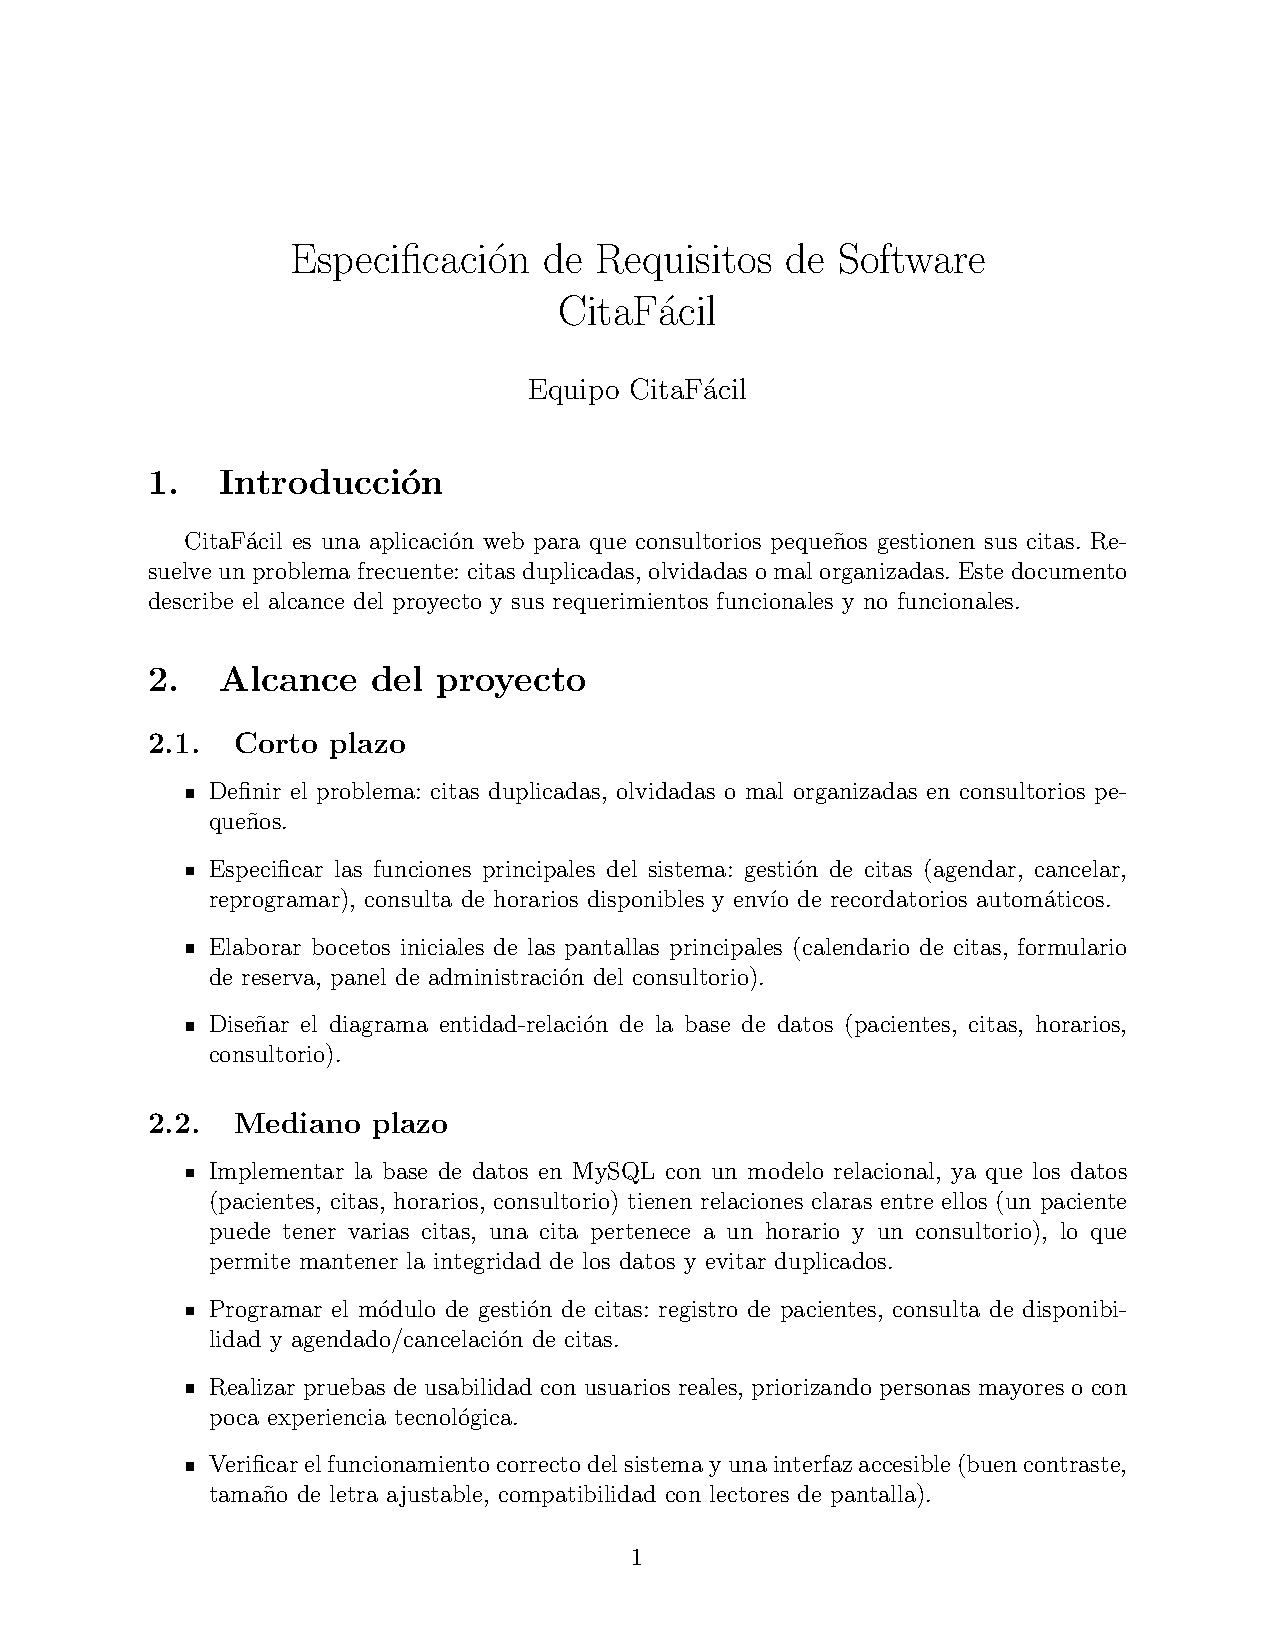
\includepdf[pages=-]{SRS.pdf}
\end{document}